\documentclass{siproblemset}

\usepackage{multicol}

% SI Session Information
\course{MTH 1321}
\sessionnum{1}
\sessiondate{1/21/21}

%\warmup{Concept Review}
\warmup{Inequalities and Intervals}
\topic{Points and Lines}
\topic{Functions and Graphs}
\topic{Quadratic Polynomials}
\topic{Trigonometric Functions}
\cooldown{Exponents and Logarithms}
%\cooldown{Rates of Change and Continuity}

% Worksheet Information
\title{Pre-Calculus Review}
%\sections{Sections 2.1-2.3}
\withnamespace

\begin{document}
    \maketitle
    
    \activity{Warmup}{Inequalities and Intervals}{Try these problems \textbf{alone} as your peers join the session.}{10 minutes}
    
    \frq{Re-write the following inequality into a single inequality of the form $a<x<b$, (i.e., in inequality notation) and draw a number line representing the inequality.}
    $$\abs{x+1}<2\text{ and }x\geq-3$$
    \smallsp
    
    \mcq[2]{Find the domain of the following functions. \textit{Recall that \underline{domain} refers to the set of numbers which answer the question ``What can I plug into this function?''}}{
        \task $g(t)=\sqrt{2-t}$
        \tinysp
        \task $f(x)=\dfrac{1}{x^2}$
        \task $f(x)=x^3$
        \tinysp
    }
    
    \activity{Activity 1}{Points and Lines}{Work together in your \textbf{breakout rooms} to answer these questions.}{10 minutes}
    
    \begin{multipartquestion}
        \frq{What is the distance formula?}
        \tinysp
        \frq{Find the distance between the points $(0,2)$ and $(-1,3)$.}
        \Smallsp
    \end{multipartquestion}

    \begin{multipartquestion}
        \frq{What is slope-intercept form? Label each part of the formula.}
        \Tinysp
        \frq{What is point-slope form? Label each part fo the formula.}
        \Tinysp
        \frq{Find the slope and y-intercept of $y=4-x$.}
        \Smallsp
        \frq{What is an equation which describes the line passing through the points $(2,0)$ and $(-1,-2)$?}
        \Smallsp
    \end{multipartquestion}

    \activity{Activity 2}{Quadratic Polynomials}{Work together in \textbf{breakout rooms} to answer these questions.}{10 minutes}
    \frq{What is the quadratic formula?}
    \tinysp
    \frq{Find the roots of $f(x)=x^2-x-1$. \textit{Recall that the ``roots'' of a function $f(x)$ are the $x$-values which make $f(x)=0$.}}
    \smallsp
    \frq{Simplify $\dfrac{x^3-64x}{x-8}$.}
    \smallsp
    
    \activity{Activity 3}{Functions and Graphs}{Answer these questions as a \textbf{large group}.}{10 minutes}
    
    \frq{Find $f\circ g$ and $g \circ f$ where $f(\theta)=2\theta$ and $g(x)=x^2+x$.}
    \Smallsp
    
    \mcq[2]{Match the following functions with their graphs below and find the values of $a$, $b$, and $m$, if applicable.}{
        \task $y=mx+b$
        \tinysp
        \task $y=ax^2+b$
        \task $y=x^3$
        \tinysp
        \task $y=b^x$
        \task $y=\log_b x$
        \tinysp
        \task $y=\sqrt{x}$
    }\newpage

    \begin{multicols}{2}
        \setlength{\parindent}{0pt}
        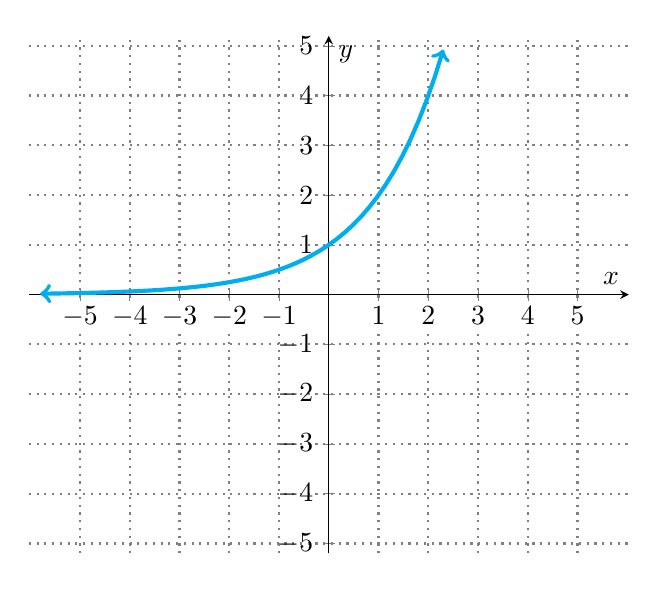
\begin{tikzpicture}
        \begin{axis}[axis x line=center, axis y line=middle,
        width=3in, %height=4in, 
        scale only axis, axis equal,
        xmin=-5.2, xmax=5.2,
        ymin=-5.2, ymax=5.2,
        xtick={-5,...,5}, ytick={-5,...,5},
        xticklabel style={draw=none, inner sep=2pt, fill=white, text opacity=1},
        xlabel={$x$}, ylabel={$y$},
        grid=both, grid style={line width=.8pt, draw=gray, dotted},
        minor tick num=0]
        \addplot[<->, cyan, line width=1.5pt, samples=50, domain=-5.8:2.3] {2^x};
        \end{axis}
        \end{tikzpicture}
        
        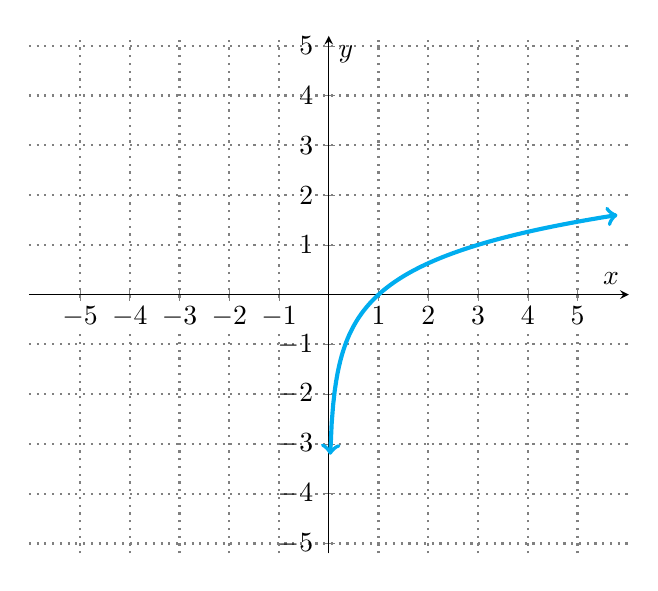
\begin{tikzpicture}
        \begin{axis}[axis x line=center, axis y line=middle,
        width=3in, %height=4in, 
        scale only axis, axis equal,
        xmin=-5.2, xmax=5.2,
        ymin=-5.2, ymax=5.2,
        xtick={-5,...,5}, ytick={-5,...,5},
        xticklabel style={draw=none, inner sep=2pt, fill=white, text opacity=1},
        xlabel={$x$}, ylabel={$y$},
        grid=both, grid style={line width=.8pt, draw=gray, dotted},
        minor tick num=0]
        \addplot[<->, cyan, line width=1.5pt, samples=200, domain=0:5.8] {ln(x)/ln(3)};
        \end{axis}
        \end{tikzpicture}
        
        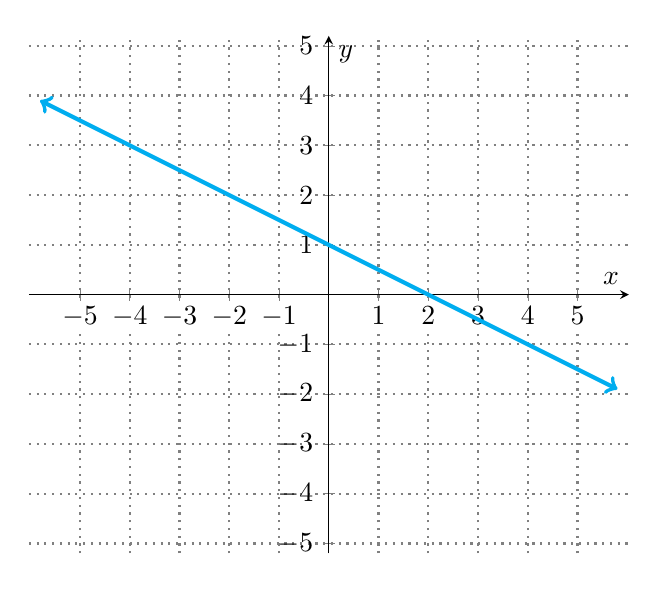
\begin{tikzpicture}
        \begin{axis}[axis x line=center, axis y line=middle,
        width=3in, %height=4in, 
        scale only axis, axis equal,
        xmin=-5.2, xmax=5.2,
        ymin=-5.2, ymax=5.2,
        xtick={-5,...,5}, ytick={-5,...,5},
        xticklabel style={draw=none, inner sep=2pt, fill=white, text opacity=1},
        xlabel={$x$}, ylabel={$y$},
        grid=both, grid style={line width=.8pt, draw=gray, dotted},
        minor tick num=0]
        \addplot[<->, cyan, line width=1.5pt, samples=50, domain=-5.8:5.8] {-1/2*x+1};
        \end{axis}
        \end{tikzpicture}
        \tinysp
        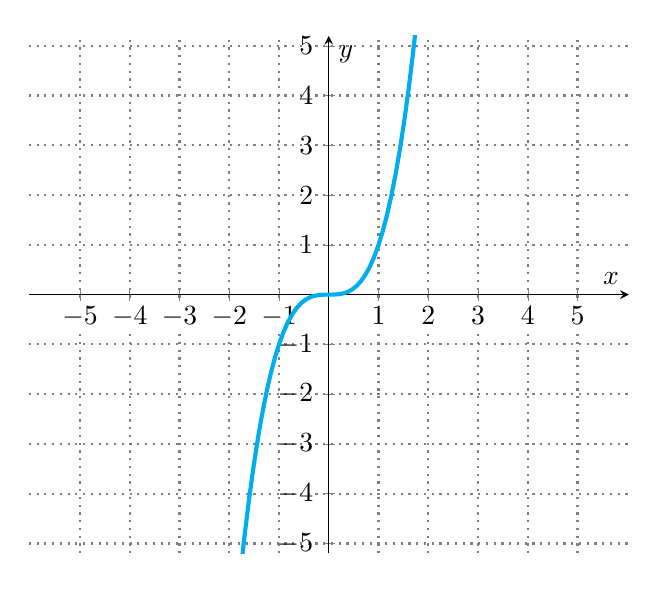
\begin{tikzpicture}
        \begin{axis}[axis x line=center, axis y line=middle,
        width=3in, %height=4in, 
        scale only axis, axis equal,
        xmin=-5.2, xmax=5.2,
        ymin=-5.2, ymax=5.2,
        xtick={-5,...,5}, ytick={-5,...,5},
        xticklabel style={draw=none, inner sep=2pt, fill=white, text opacity=1},
        xlabel={$x$}, ylabel={$y$},
        grid=both, grid style={line width=.8pt, draw=gray, dotted},
        minor tick num=0]
        \addplot[<->, cyan, line width=1.5pt, samples=50, domain=-2.12:2.12] {x^3};
        \end{axis}
        \end{tikzpicture}
        \tinysp
        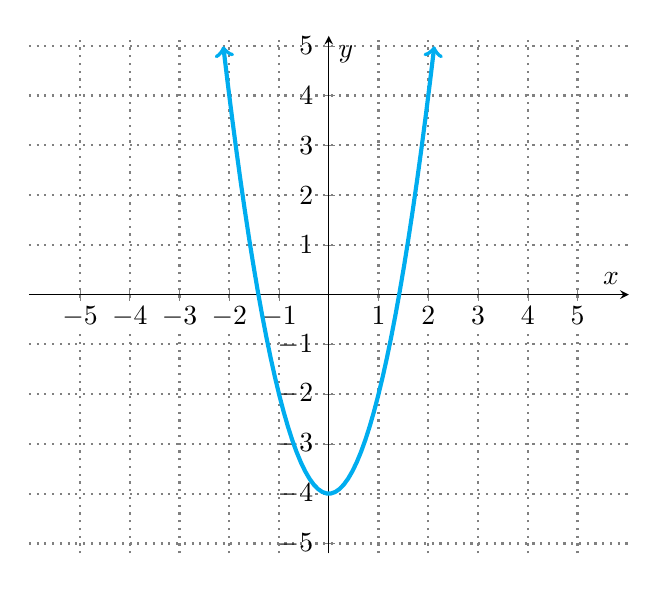
\begin{tikzpicture}
        \begin{axis}[axis x line=center, axis y line=middle,
        width=3in, %height=4in, 
        scale only axis, axis equal,
        xmin=-5.2, xmax=5.2,
        ymin=-5.2, ymax=5.2,
        xtick={-5,...,5}, ytick={-5,...,5},
        xticklabel style={draw=none, inner sep=2pt, fill=white, text opacity=1},
        xlabel={$x$}, ylabel={$y$},
        grid=both, grid style={line width=.8pt, draw=gray, dotted},
        minor tick num=0]
        \addplot[<->, cyan, line width=1.5pt, samples=50, domain=-2.12:2.12] {2*x^2-4};
        \end{axis}
        \end{tikzpicture}
        \tinysp
        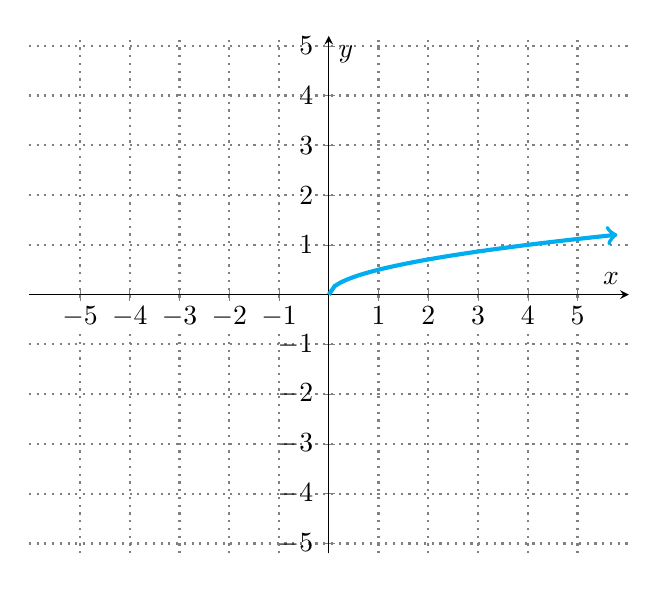
\begin{tikzpicture}
        \begin{axis}[axis x line=center, axis y line=middle,
        width=3in, %height=4in, 
        scale only axis, axis equal,
        xmin=-5.2, xmax=5.2,
        ymin=-5.2, ymax=5.2,
        xtick={-5,...,5}, ytick={-5,...,5},
        xticklabel style={draw=none, inner sep=2pt, fill=white, text opacity=1},
        xlabel={$x$}, ylabel={$y$},
        grid=both, grid style={line width=.8pt, draw=gray, dotted},
        minor tick num=0]
        \addplot[->, cyan, line width=1.5pt, samples=50, domain=0:5.8] {sqrt(x)/2};
        \end{axis}
        \end{tikzpicture}
        \tinysp
    \end{multicols}
    \newpage
    
    \begin{multicols}{2}
        \activity{Activity 4}{Exponents}{Work together in your \textbf{breakout rooms} to answer these questions.}{10 minutes}
        $$a^{b/c}=\sqrt[c]{a^b}=(\sqrt[c]{a})^b$$
        \vspace{-0.8cm}
        \begin{multipartquestion}
            Complete the following identities.
            \frq{$\paren{a^b}^c=$}
            \tinysp
            \frq{$a^ba^c=$}
            \tinysp
            \frq{$\dfrac{a^b}{a^c}=$}
            \tinysp
        \end{multipartquestion}
%        \frq{Solve for $x$:}
%        $$\dfrac{1}{27}=x^{-3/2}$$
%        \Normalsp
        \frq{Simplify:}
        $$(2^34^2)^{1/2}$$
        \smallsp
        \frq{Simplify:}
        $$8^{3\log_82}$$
        \vfill\null
        \columnbreak
        \activity{Activity 5}{Logarithms}{Work together in your \textbf{breakout rooms} to answer these questions.}{10 minutes}
        $$a^b=c \Rightarrow \log_b(c)=a$$
        \vspace{-0.9cm}
        \begin{multipartquestion}
            Complete the following identities.
            \frq{$\log(a^b)=$}
            \tinysp
            \frq{$\log(ab)=$}
            \tinysp
            \frq{$\log\left(\dfrac{a}{b}\right)=$}
            \tinysp
            \frq{$b^{\log_bx}=\log_b(b^x)=$}
            \tinysp
            \frq{$\log_bb=$}
            \tinysp
            \frq{$\log_b1=$}
            \tinysp
        \end{multipartquestion}
        \mcq{Simplify the following expressions.}{
            \task $\log_448-\log_412$
            \smallsp
            \task $2\ln5+3\ln4$
        }
        \vfill\null
    \end{multicols}

    \newpage
    
    \activity{Cooldown}{Trigonometric Functions}{Answer these questions as a \textbf{large group}.}{15 minutes}

    \begin{tikzpicture}[scale=5.3,cap=round,>=latex, every node/.style={scale=1.3}]
    % draw the coordinates
    \draw[->] (-1.5cm,0cm) -- (1.5cm,0cm) node[right,fill=white] {$x$};
    \draw[->] (0cm,-1.5cm) -- (0cm,1.5cm) node[above,fill=white] {$y$};
    
    % draw the unit circle
    \draw[thick] (0cm,0cm) circle(1cm);
    
    \foreach \x in {0,30,...,360} {
        % lines from center to point
        \draw[gray] (0cm,0cm) -- (\x:1cm);
        % dots at each point
        \filldraw[black] (\x:1cm) circle(0.4pt);
        % draw each angle in degrees
        \draw (\x:0.6cm) node[fill=white] {$\x^\circ$};
    }

    \foreach \x in {45,135,225,315} {
        % lines from center to point
        \draw[gray] (0cm,0cm) -- (\x:1cm);
        % dots at each point
        \filldraw[black] (\x:1cm) circle(0.4pt);
        % draw each angle in degrees
        \draw (\x:0.6cm) node[fill=white] {$\x^\circ$};
    }
    
    % draw each angle in radians
    \foreach \x/\xtext in {
        30/\frac{\pi}{6},
        45/\frac{\pi}{4},
        60/\frac{\pi}{3},
        90/\frac{\pi}{2},
        120/\frac{2\pi}{3},
        135/\frac{3\pi}{4},
        150/\frac{5\pi}{6},
        180/\pi,
        210/\frac{7\pi}{6},
        225/\frac{5\pi}{4},
        240/\frac{4\pi}{3},
        270/\frac{3\pi}{2},
        300/\frac{5\pi}{3},
        315/\frac{7\pi}{4},
        330/\frac{11\pi}{6},
        360/2\pi}
    \draw (\x:0.85cm) node[fill=white] {$\hspace{.25in}$};
    
    \foreach \x/\xtext/\y in {
        % the coordinates for the first quadrant
        30/\hspace{.25in}/\hspace{.25in},
        45/\hspace{.25in}/\hspace{.25in},
        60/\hspace{.25in}/\hspace{.25in},
        % the coordinates for the second quadrant
        150/\hspace{.25in}/\hspace{.25in},
        135/\hspace{.25in}/\hspace{.25in},
        120/\hspace{.25in}/\hspace{.25in},
        % the coordinates for the third quadrant
        210/\hspace{.25in}/\hspace{.25in},
        225/\hspace{.25in}/\hspace{.25in},
        240/\hspace{.25in}/\hspace{.25in},
        % the coordinates for the fourth quadrant
        330/\hspace{.25in}/\hspace{.25in},
        315/\hspace{.25in}/\hspace{.25in},
        300/\hspace{.25in}/\hspace{.25in}}
    \draw (\x:1.25cm) node {$\left(\xtext,\y\right)$};
    
    % draw the horizontal and vertical coordinates
    % the placement is better this way
    \draw (-1.25cm,0cm) node[above=1pt] {$(\hspace{.25in},\hspace{.25in})$}
    (1.25cm,0cm)  node[above=1pt] {$(\hspace{.25in},\hspace{.25in})$}
    (0cm,-1.25cm) node[fill=white] {$(\hspace{.25in},\hspace{.25in})$}
    (0cm,1.25cm)  node[fill=white] {$(\hspace{.25in},\hspace{.25in})$};
    \end{tikzpicture}
    \newpage
    
    \frq{Complete the following identities.}
    \begin{center}
        \begin{tabular}{c c}
            $\sin=\dfrac{1}{\hspace{1in}}=\dfrac{\hspace{0.5in}}{\hspace{0.5in}}$\tinysp & 
            $\csc=\dfrac{1}{\hspace{1in}}=\dfrac{\hspace{0.5in}}{\hspace{0.5in}}$ \\
            $\cos=\dfrac{1}{\hspace{1in}}=\dfrac{\hspace{0.5in}}{\hspace{0.5in}}$\tinysp & 
            $\sec=\dfrac{1}{\hspace{1in}}=\dfrac{\hspace{0.5in}}{\hspace{0.5in}}$ \\
            $\tan=\dfrac{1}{\hspace{1in}}=\dfrac{\hspace{1in}}{\hspace{1in}}=\dfrac{\hspace{0.5in}}{\hspace{0.5in}}$ &
            $\cot=\dfrac{1}{\hspace{1in}}=\dfrac{\hspace{1in}}{\hspace{1in}}=\dfrac{\hspace{0.5in}}{\hspace{0.5in}}$ \\
        \end{tabular}
    \end{center}
    
    \mcq{Find $\theta$ such that}{
        \task $\cos \theta=\frac{\sqrt{3}}{2}$
        \Tinysp
        \task $\csc \theta=2$
    }
    \newpage
    
    
    
\end{document}